%! Author = Saeid Yazdani
%! Date = 8/18/2024


\section{System Module Add-In Cards}
\label{ch:system-boards}

In this section, the module (add-in) cards that form the system on a backplane
will be introduced and their most important input and output signal connections
to the backplane will be presented.

%%%%%%%%%%%%%%%%%%%%%%%%%%%%%%%%%%%%%%%%%%%%%%%%%%%%%%%%%%%%%%%%%%%%%%%%%%%%%%%%
%%%%%%%%%%%%%%%%%%%%%%%%%%%%%%%%%%%%%%%%%%%%%%%%%%%%%%%%%%%%%%%%%%%%%%%%%%%%%%%%

\subsection{Tracking-Supply Board}
\label{subsec:tracking-Supply-board}

Two tracking-supply boards are responsible for generating positive and
negative voltage rails (max \SI{\pm350}{\volt}) for the source follower and
\SI{5}{\volt} system voltage from mains (\SI{24}{\V}/\SI{10}{\ampere})
DC power supply\footnote{Mean Well LRS-100-24.}.
These boards are identical and selecting a jumper can configure the boards for
either positive or negative output.
\autoref{fig:tracking-supply-figure} shows the prototype board and its
block diagram respectively where the important building blocks are annotated.

\begin{figure}[!htb]
    \centering
    \begin{subfigure}[b]{\textwidth}
        \centering
        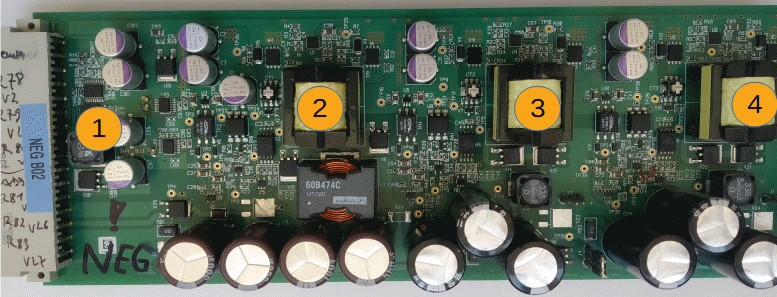
\includegraphics[width=\linewidth,height=0.30\textheight,keepaspectratio]{figures/prototype/production/tracking-supply-board}
        \caption{
            Tracking-Supply Board \acs{PCB}.
            \textbf{(1)} Switching DC/DC regulator for \SI{5}{\volt} system voltage (not isolated).
            \textbf{(2)} First (primary) adjustable isolated switching DC/DC regulator \SI{0}{\volt} to \SI{55}{\volt} (always on).
            \textbf{(3)} Second series regulator \SI{0}{\volt} to \SI{150}{\volt}.
            \textbf{(4)} Third series regulator \SI{0}{\volt} to \SI{150}{\volt}.
        }
        \label{fig:subfig1}
    \end{subfigure}

    \vspace{0.4em}

    \begin{subfigure}[b]{\textwidth}
        \centering
        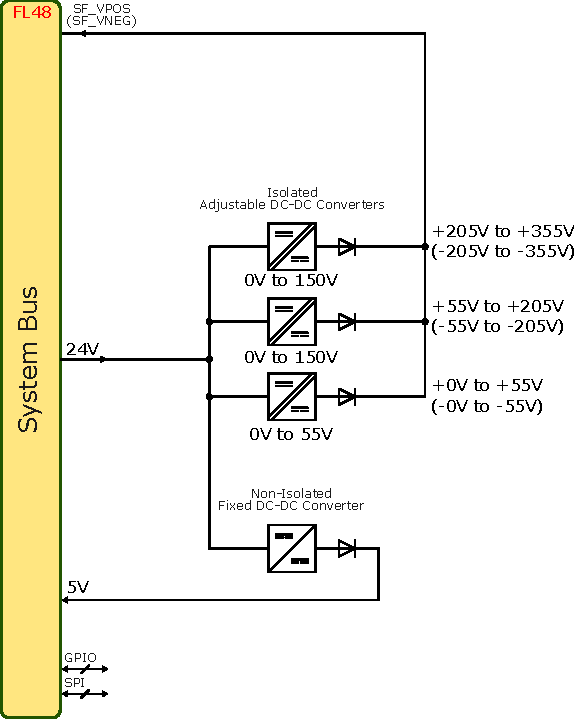
\includegraphics[width=\linewidth,height=0.44\textheight,keepaspectratio]{figures/prototype/tracking-supply-board-diagram}
        \caption{Tracking-Supply Board Diagram.}
        \label{fig:subfig2}
    \end{subfigure}

    \caption[Tracking-Supply Board Module]{
        Tracking-Supply module.
    }
    \label{fig:tracking-supply-figure}
\end{figure}

%%%%%%%%%%%%%%%%%%%%%%%%%%%%%%%%%%%%%%%%%%%%%%%%%%%%%%%%%%%%%%%%%%%%%%%%%%%%%%%%
%%%%%%%%%%%%%%%%%%%%%%%%%%%%%%%%%%%%%%%%%%%%%%%%%%%%%%%%%%%%%%%%%%%%%%%%%%%%%%%%

\subsection{Controller Board}
\label{subsec:controller-board}

The controller board provides the processing power for control loop algorithms,
system management (relays, LEDs, etc.)
and the communication to the outside world (e.g. a \acs{PC} or an
\ac{ATE}) using USB or Serial interface.
\autoref{fig:controller-board} shows the prototype board and its
block diagram, respectively, where the important building blocks are annotated.

\begin{figure}[!htb]
    \centering
    \begin{subfigure}[b]{\textwidth}
        \centering
        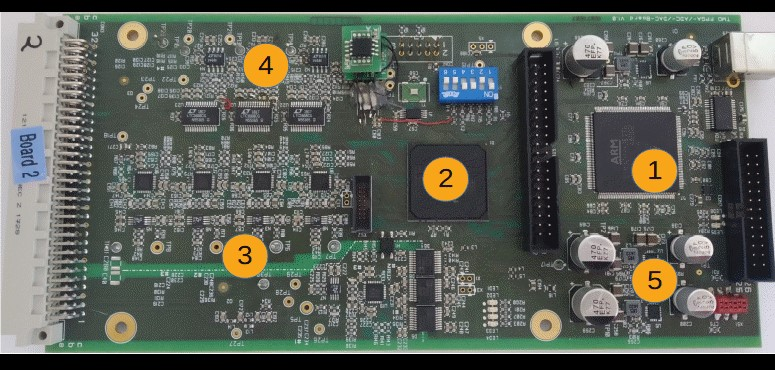
\includegraphics[width=\linewidth,height=0.30\textheight,keepaspectratio]{figures/prototype/production/controller-board}
        \caption{Controller Board \acs{PCB}.
        \textbf{(1)} The microcontroller (STM32H7), USB and serial connectors.
        \textbf{(2)} The FPGA (CycloneV) and program flash chip.
        \textbf{(3)} Five \ac{ADC} chips for voltage and current measurements.
        \textbf{(4)} Three \ac{DAC} chips for set-point, coarse and vernier values.
        \textbf{(5)} Local switching regulator used for MCU and FPGA chips.
        }
        \label{fig:subfig1}
    \end{subfigure}

    \vspace{0.4em}

    \begin{subfigure}[b]{\textwidth}
        \centering
        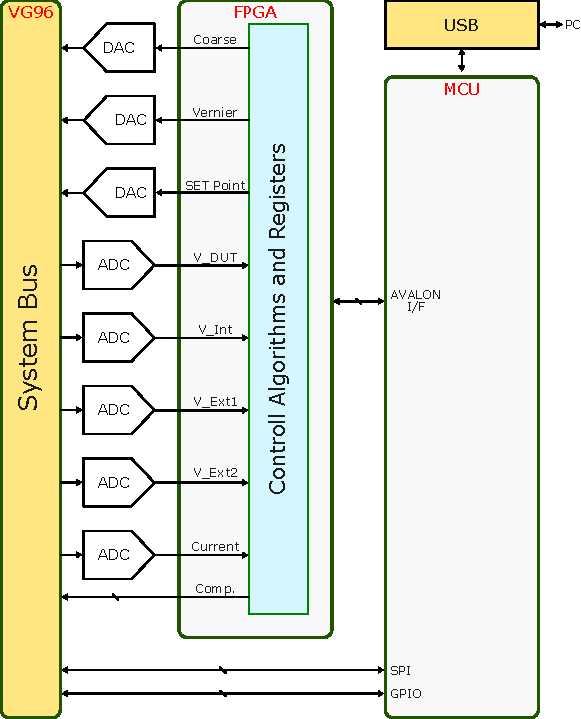
\includegraphics[width=\linewidth,height=0.44\textheight,keepaspectratio]{figures/prototype/controller-board-block-diagram}
        \caption{Controller Board Diagram.}
        \label{fig:subfig2}
    \end{subfigure}

    \caption[Controller Board Module]{
        Controller Board module.
    }
    \label{fig:controller-board}
\end{figure}

%%%%%%%%%%%%%%%%%%%%%%%%%%%%%%%%%%%%%%%%%%%%%%%%%%%%%%%%%%%%%%%%%%%%%%%%%%%%%%%%
%%%%%%%%%%%%%%%%%%%%%%%%%%%%%%%%%%%%%%%%%%%%%%%%%%%%%%%%%%%%%%%%%%%%%%%%%%%%%%%%

\subsection{Monitor Board}
\label{subsec:Monitor-board}

The monitor board is mainly intended for debugging purposes thanks to two
DACs that deliver signals equal to the output voltage and the output current
on standard \acs{BNC} connectors where these signals can be observed by an
oscilloscope or network analyzer.
In addition, the extra space is used for placing more switching regulators for
internal components.
\autoref{fig:monitor-board} shows the prototype board and its
block diagram, respectively, where the important building blocks are annotated.

\begin{figure}[!htb]
    \centering
    \begin{subfigure}[b]{\textwidth}
        \centering
        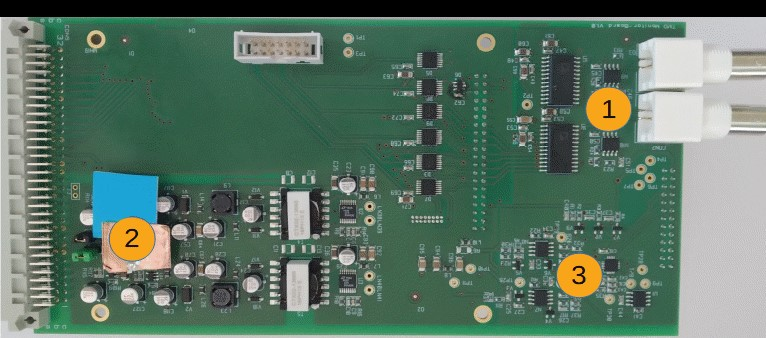
\includegraphics[width=\linewidth,height=0.30\textheight,keepaspectratio]{figures/prototype/production/monitor-board}
        \caption{Monitor Board \acs{PCB}.
        \textbf{(1)} Voltage and current debug \acp{DAC} and \acs{BNC} connectors.
        \textbf{(2)} Local voltage regulators for \SI{\pm15}{\volt} and \SI{\pm5}{\volt}
        used by internal components.
        \textbf{(3)} \ac{ADC} for measuring selected internal voltages (self-test) of the
        whole system by accessing backplane bus voltages.
        }
        \label{fig:subfig1}
    \end{subfigure}

    \vspace{0.4em}

    \begin{subfigure}[b]{\textwidth}
        \centering
        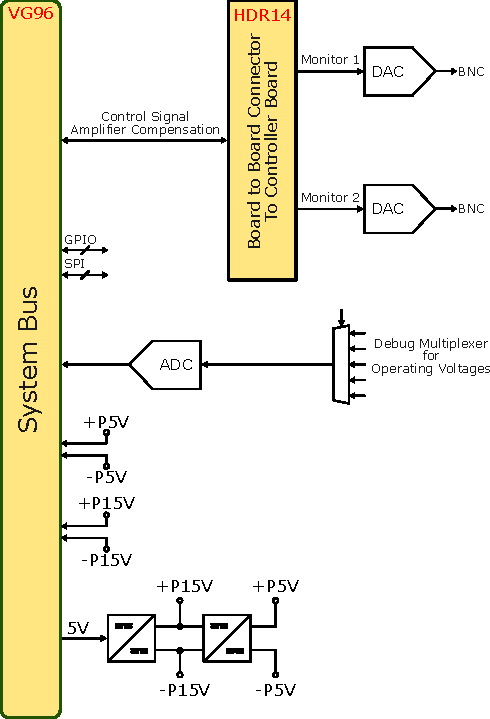
\includegraphics[width=\linewidth,height=0.44\textheight,keepaspectratio]{figures/prototype/monitor-board-block-diagram}
        \caption{Monitor Board Diagram.}
        \label{fig:subfig2}
    \end{subfigure}

    \caption[Monitor Board Module]{
        Monitor Board module.
    }
    \label{fig:monitor-board}
\end{figure}

%%%%%%%%%%%%%%%%%%%%%%%%%%%%%%%%%%%%%%%%%%%%%%%%%%%%%%%%%%%%%%%%%%%%%%%%%%%%%%%%
%%%%%%%%%%%%%%%%%%%%%%%%%%%%%%%%%%%%%%%%%%%%%%%%%%%%%%%%%%%%%%%%%%%%%%%%%%%%%%%%

\subsection{Frontend Board}
\label{subsec:frontend-board}

The frontend board contains output measurement and power delivery circuits.
Current shunt resistor arrays for current sensing and voltage dividers for
voltage measurements are on this board.
\autoref{fig:frontend-board} shows the prototype board and its
block diagram, respectively, where the important building blocks are annotated.

\begin{figure}[!htb]
    \centering
    \begin{subfigure}[b]{\textwidth}
        \centering
        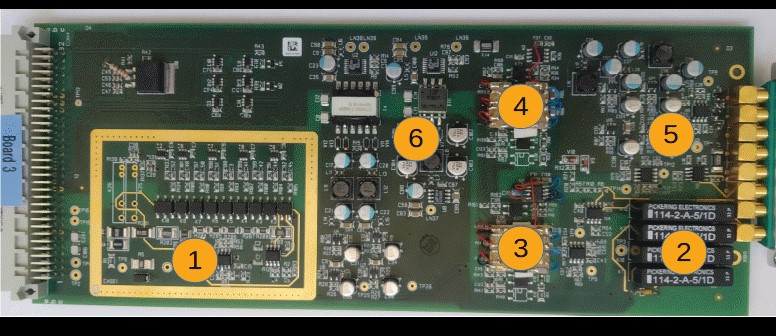
\includegraphics[width=\linewidth,height=0.30\textheight,keepaspectratio]{figures/prototype/production/frontend-board}
        \caption{Frontend Board \acs{PCB}.
        \textbf{(1)} Current measurement block containing shunt resistors
        and their associated \acp{SSR}, current source amplifier,
            buffer amplifier and guard ring (exposed gold PCB traces).
            \textbf{(2)}
            PIN Relay for engaging/disengaging the output.
            \textbf{(3)}
            \acs{DUT} Voltage measurement with buffer, resistor divider network
            for range selection and differential amplifier.
            \textbf{(4)}
            Internal voltage measurement block with the same feature as \acs{DUT}
            voltage measurement.
            \textbf{(5)}
            Input buffer for modulated input.
            \textbf{(6)}
            Local floating switching power supply for current measurement block
            providing \SI{\pm15}{\volt}, \SI{\pm5}{\volt} and \SI{\pm2.5}{\volt}.
        }
        \label{fig:subfig1}
    \end{subfigure}

    \vspace{0.4em}

    \begin{subfigure}[b]{\textwidth}
        \centering
        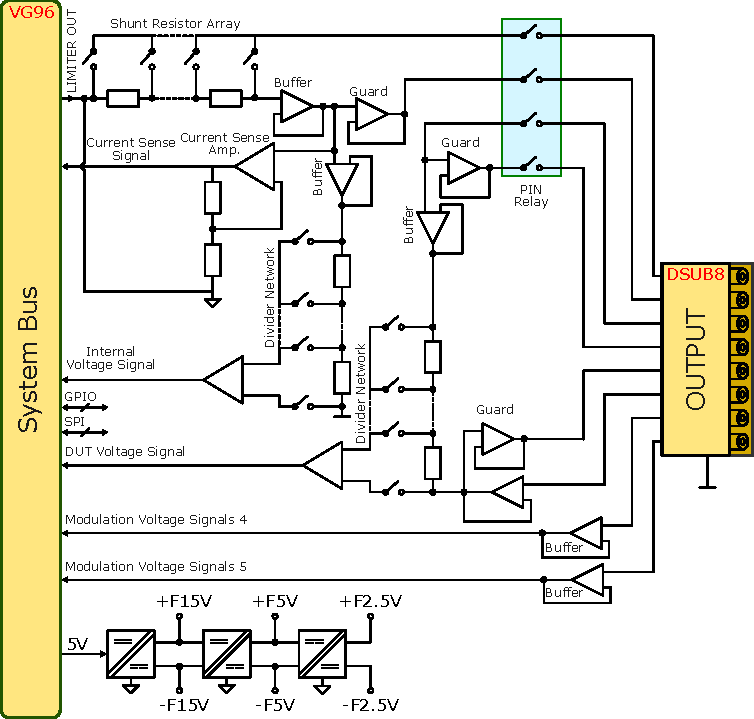
\includegraphics[width=\linewidth,height=0.44\textheight,keepaspectratio]{figures/prototype/frontend-board-block-diagram}
        \caption{Frontend Board Diagram.}
        \label{fig:subfig2}
    \end{subfigure}

    \caption[Frontend Board Module]{
        Frontend Board module.
    }
    \label{fig:frontend-board}
\end{figure}

%%%%%%%%%%%%%%%%%%%%%%%%%%%%%%%%%%%%%%%%%%%%%%%%%%%%%%%%%%%%%%%%%%%%%%%%%%%%%%%%
%%%%%%%%%%%%%%%%%%%%%%%%%%%%%%%%%%%%%%%%%%%%%%%%%%%%%%%%%%%%%%%%%%%%%%%%%%%%%%%%

\FloatBarrier

\subsection{Amplifier Board}
\label{subsec:amplifier-board}

As discussed in \autoref{sec:output-driver-stage}, the amplifier board
contains the three-stage output driver as well as the compensation networks for
pre and power amplifiers.
\autoref{fig:amplifier-board} shows the prototype board and its
block diagram, respectively, where the important building blocks are annotated:

\begin{figure}[!htb]
    \centering
    \begin{subfigure}[b]{\textwidth}
        \centering
        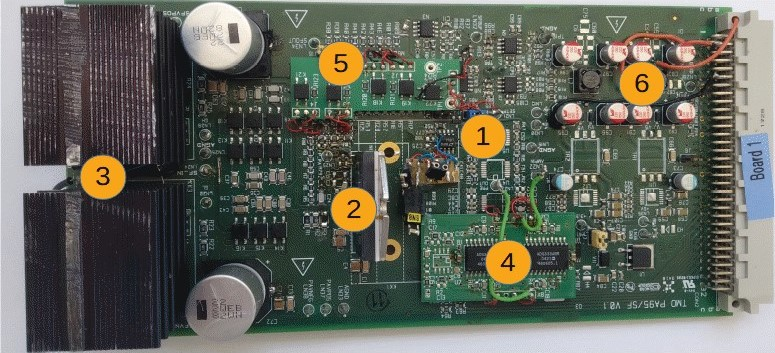
\includegraphics[width=\linewidth,height=0.30\textheight,keepaspectratio]{figures/prototype/production/amplifier-board}
        \caption{Amplifier Board \acs{PCB}.
        \textbf{(1)} Summing and pre amplifier.
        \textbf{(2)}
        PA95 Power Amplifier.
        \textbf{(3)}
        Current booster arrangement with heatsinks.
        \textbf{(4)}
        Compensation networks.
        \textbf{(5)}
        Gain setting network for the power amplifier.
        \textbf{(6)}
        Local floating switching power supply for the power amplifier (PA95)
            \SI{\pm25}{\volt}.
        }
        \label{fig:subfig1}
    \end{subfigure}

    \vspace{0.4em}

    \begin{subfigure}[b]{\textwidth}
        \centering
        
\includegraphics[width=\linewidth,height=0.44\textheight,keepaspectratio]{{figures/prototype/amplifier-board-block-diagram}}
        \caption{Amplifier Board Diagram.}
        \label{fig:subfig2}
    \end{subfigure}

    \caption[Amplifier Board Module]{
        Amplifier Board module.
    }
    \label{fig:amplifier-board}
\end{figure}

%%%%%%%%%%%%%%%%%%%%%%%%%%%%%%%%%%%%%%%%%%%%%%%%%%%%%%%%%%%%%%%%%%%%%%%%%%%%%%%%
%%%%%%%%%%%%%%%%%%%%%%%%%%%%%%%%%%%%%%%%%%%%%%%%%%%%%%%%%%%%%%%%%%%%%%%%%%%%%%%%
\FloatBarrier

\subsection{System Integration}
\label{subsec:system-integration}

\autoref{fig:dps-modules-inserted} shows the integration of
the \acs{HVS} system where all modules are inserted into the backplane within
a standard 19 inch rack where \autoref{fig:dps-with-backplane} shows the
another view where a few of the modules are removed to expose the backplane.

The following list identifies system modules as presented in
\autoref{fig:dps-modules-inserted}:

\begin{enumerate}[topsep=8pt,itemsep=4pt,partopsep=4pt, parsep=4pt]
    \item Controller Board.

    \item Monitor Board (with USB cable attached).

    \item Frontend Board (with output cable DSUB8 attached).

    \item Limiter Board.

    \item Amplifier Board.

    \item Positive Tracking Supply Board.

    \item Negative Tracking Supply Board.

    \item Mains plug and master switch.

\end{enumerate}

\begin{figure}[htp]
    \centering
    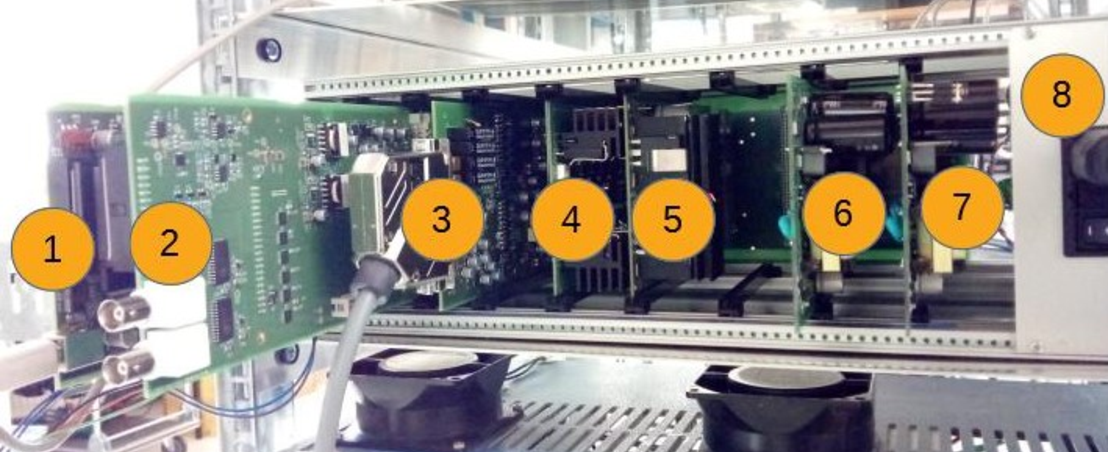
\includegraphics[width=\textwidth]
    {figures/prototype/dps-in-rack}
    \caption[Modules Inserted in Backplane]{
        The \acs{HVS} system after integration of all modules and backplane
        in a 19-Inch rack.
    }
    \label{fig:dps-modules-inserted}
\end{figure}

\begin{figure}[htp]
    \centering
    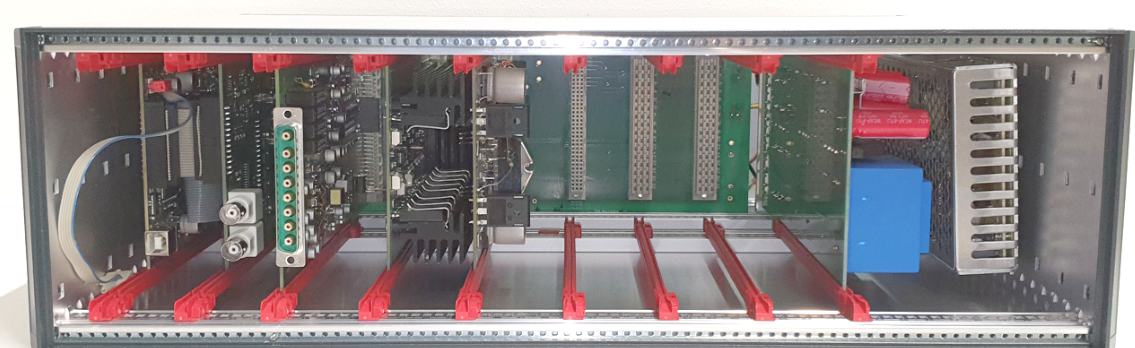
\includegraphics[width=\textwidth]
    {figures/prototype/dps-with-backplane}
    \caption[Backplane View]{
        Backplane View. A Few of the boards are removed to expose the backplane.
    }
    \label{fig:dps-with-backplane}
\end{figure}


